\hbadness = 10001
\vbadness = 10001
\documentclass[journal,12pt,twocolumn]{IEEEtran}
\usepackage{setspace}
\usepackage{textcomp}
\usepackage{gensymb}
\usepackage{xcolor}
\usepackage{caption}
%\usepackage{subcaption}
%\doublespacing
\singlespacing
%\usepackage{graphicx}
%\usepackage{amssymb}
%\usepackage{relsize}
\usepackage[cmex10]{amsmath}
\usepackage{mathtools}
%\usepackage{amsthm}
%\interdisplaylinepenalty=2500
%\savesymbol{iint}
%\usepackage{txfonts}
%\restoresymbol{TXF}{iint}
%\usepackage{wasysym}
\usepackage{hyperref}
\usepackage{amsthm}
\usepackage{mathrsfs}
\usepackage{txfonts}
\usepackage{stfloats}
\usepackage{cite}
\usepackage{cases}
\usepackage{subfig}
%\usepackage{xtab}
\usepackage{longtable}
\usepackage{multirow}
%\usepackage{algorithm}
%\usepackage{algpseudocode}
%\usepackage{enumerate}
\usepackage{enumitem}
\usepackage{mathtools}
%\usepackage{iithtlc}
%\usepackage[framemethod=tikz]{mdframed}
\usepackage{listings}
\let\vec\mathbf
%\usepackage{stmaryrd}
%\usepackage{wasysym}
%\newcounter{MYtempeqncnt}
\DeclareMathOperator*{\Res}{Res}
%\renewcommand{\baselinestretch}{2}
\renewcommand\thesection{\arabic{section}}
\renewcommand\thesubsection{\thesection.\arabic{subsection}}
\renewcommand\thesubsubsection{\thesubsection.\arabic{subsubsection}}
\renewcommand\thesectiondis{\arabic{section}}
\renewcommand\thesubsectiondis{\thesectiondis.\arabic{subsection}}
\renewcommand\thesubsubsectiondis{\thesubsectiondis.\arabic{subsubsection}}
%\renewcommand{\labelenumi}{\textbf{\theenumi}}
%\renewcommand{\theenumi}{P.\arabic{enumi}}
% correct bad hyphenation here
\hyphenation{op-tical net-works semi-conduc-tor}
\lstset{
language=Python,
frame=single, 
breaklines=true,
columns=fullflexible
}
\begin{document}
%
\theoremstyle{definition}
\newtheorem{theorem}{Theorem}[section]
\newtheorem{problem}{Problem}
\newtheorem{proposition}{Proposition}[section]
\newtheorem{lemma}{Lemma}[section]
\newtheorem{corollary}[theorem]{Corollary}
\newtheorem{example}{Example}[section]
\newtheorem{definition}{Definition}[section]
%\newtheorem{algorithm}{Algorithm}[section]
%\newtheorem{cor}{Corollary}
\newcommand{\BEQA}{\begin{eqnarray}}
\newcommand{\EEQA}{\end{eqnarray}}
\newcommand{\define}{\stackrel{\triangle}{=}}
\newcommand{\myvec}[1]{\ensuremath{\begin{pmatrix}#1\end{pmatrix}}}
\newcommand{\mydet}[1]{\ensuremath{\begin{vmatrix}#1\end{vmatrix}}}
\bibliographystyle{IEEEtran}
%\bibliographystyle{ieeetr}
\providecommand{\nCr}[2]{\,^{#1}C_{#2}} % nCr
\providecommand{\nPr}[2]{\,^{#1}P_{#2}} % nPr
\providecommand{\mbf}{\mathbf}
\providecommand{\pr}[1]{\ensuremath{\Pr\left(#1\right)}}
\providecommand{\qfunc}[1]{\ensuremath{Q\left(#1\right)}}
\providecommand{\sbrak}[1]{\ensuremath{{}\left[#1\right]}}
\providecommand{\lsbrak}[1]{\ensuremath{{}\left[#1\right.}}
\providecommand{\rsbrak}[1]{\ensuremath{{}\left.#1\right]}}
\providecommand{\brak}[1]{\ensuremath{\left(#1\right)}}
\providecommand{\lbrak}[1]{\ensuremath{\left(#1\right.}}
\providecommand{\rbrak}[1]{\ensuremath{\left.#1\right)}}
\providecommand{\cbrak}[1]{\ensuremath{\left\{#1\right\}}}
\providecommand{\lcbrak}[1]{\ensuremath{\left\{#1\right.}}
\providecommand{\rcbrak}[1]{\ensuremath{\left.#1\right\}}}
\theoremstyle{remark}
\newtheorem{rem}{Remark}
\newcommand{\sgn}{\mathop{\mathrm{sgn}}}
\providecommand{\abs}[1]{\left\vert#1\right\vert}
\providecommand{\res}[1]{\Res\displaylimits_{#1}} 
\providecommand{\norm}[1]{\lVert#1\rVert}
\providecommand{\mtx}[1]{\mathbf{#1}}
\providecommand{\mean}[1]{E\left[ #1 \right]}
\providecommand{\fourier}{\overset{\mathcal{F}}{ \rightleftharpoons}}
\providecommand{\ztrans}{\overset{\mathcal{Z}}{ \rightleftharpoons}}
%\providecommand{\hilbert}{\overset{\mathcal{H}}{ \rightleftharpoons}}
\providecommand{\system}{\overset{\mathcal{H}}{ \longleftrightarrow}}
	%\newcommand{\solution}[2]{\textbf{Solution:}{#1}}
\newcommand{\solution}{\noindent \textbf{Solution: }}
\providecommand{\dec}[2]{\ensuremath{\overset{#1}{\underset{#2}{\gtrless}}}}
\numberwithin{equation}{section}
%\numberwithin{equation}{subsection}
%\numberwithin{problem}{subsection}
%\numberwithin{definition}{subsection}
\makeatletter
\@addtoreset{figure}{problem}
\makeatother

\let\StandardTheFigure\thefigure
%\renewcommand{\thefigure}{\theproblem.\arabic{figure}}
\renewcommand{\thefigure}{\theproblem}
%\numberwithin{figure}{subsection}
\def\putbox#1#2#3{\makebox[0in][l]{\makebox[#1][l]{}\raisebox{\baselineskip}[0in][0in]{\raisebox{#2}[0in][0in]{#3}}}}
     \def\rightbox#1{\makebox[0in][r]{#1}}
     \def\centbox#1{\makebox[0in]{#1}}
     \def\topbox#1{\raisebox{-\baselineskip}[0in][0in]{#1}}
     \def\midbox#1{\raisebox{-0.5\baselineskip}[0in][0in]{#1}}
\vspace{3cm}

\title{ 
%\logo{
%}
Pingala Series
%	\logo{Octave for Math Computing }
}
%\title{
%	\logo{Matrix Analysis through Octave}{\begin{center}\includegraphics[scale=.24]{tlc}\end{center}}{}{HAMDSP}
%}
% paper title
% can use linebreaks \\ within to get better formatting as desired
%\title{Matrix Analysis through Octave}
%
%
% author names and IEEE memberships
% note positions of commas and nonbreaking spaces ( ~ ) LaTeX will not break
% a structure at a ~ so this keeps an author's name from being broken across
% two lines.
% use \thanks{} to gain access to the first footnote area
% a separate \thanks must be used for each paragraph as LaTeX2e's \thanks
% was not built to handle multiple paragraphs
%
\author{ G V V Sharma$^{*}$ %<-this  stops a space
\thanks{*The author is with the Department
of Electrical Engineering, Indian Institute of Technology, Hyderabad
502285 India e-mail:  gadepall@iith.ac.in.  All content in the manuscript is 
released under GNU GPL.  Free to use for anything. }% <-this % stops a space
%\thanks{J. Doe and J. Doe are with Anonymous University.}% <-this % stops a space
%\thanks{Manuscript received April 19, 2005; revised January 11, 2007.}}
}
% note the % following the last \IEEEmembership and also \thanks - 
% these prevent an unwanted space from occurring between the last author name
% and the end of the author line. i.e., if you had this:
% 
% \author{....lastname \thanks{...} \thanks{...} }
%                     ^------------^------------^----Do not want these spaces!
%
% a space would be appended to the last name and could cause every name on that
% line to be shifted left slightly. This is one of those "LaTeX things". For
% instance, "\textbf{A} \textbf{B}" will typeset as "A B" not "AB". To get
% "AB" then you have to do: "\textbf{A}\textbf{B}"
% \thanks is no different in this regard, so shield the last } of each \thanks
% that ends a line with a % and do not let a space in before the next \thanks.
% Spaces after \IEEEmembership other than the last one are OK (and needed) as
% you are supposed to have spaces between the names. For what it is worth,
% this is a minor point as most people would not even notice if the said evil
% space somehow managed to creep in.

% The paper headers
%\markboth{Journal of \LaTeX\ Class Files,~Vol.~6, No.~1, January~2007}%
%{Shell \MakeLowercase{\textit{et al.}}: Bare Demo of IEEEtran.cls for Journals}
% The only time the second header will appear is for the odd numbered pages
% after the title page when using the twoside option.
% 
% *** Note that you probably will NOT want to include the author's ***
% *** name in the headers of peer review papers.                   ***
% You can use \ifCLASSOPTIONpeerreview for conditional compilation here if
% you desire.
% If you want to put a publisher's ID mark on the page you can do it like
% this:
%\IEEEpubid{0000--0000/00\$00.00~\copyright~2007 IEEE}
% Remember, if you use this you must call \IEEEpubidadjcol in the second
% column for its text to clear the IEEEpubid mark.
% make the title area
\maketitle
%\newpage
\tableofcontents
%\renewcommand{\thefigure}{\thesection.\theenumi}
%\renewcommand{\thetable}{\thesection.\theenumi}
\renewcommand{\thefigure}{\theenumi}
\renewcommand{\thetable}{\theenumi}
%\renewcommand{\theequation}{\thesection}
\bigskip

\begin{abstract}
This manual provides a simple introduction to Transforms
\end{abstract}
\section{JEE 2019}
Let 
\begin{align}
	a_n &= \frac{\alpha^{n}-\beta^{n}}{\alpha - \beta}, \quad n \ge 1
	\\
	b_n &= a_{n-1} + a_{n+1}, \quad n \ge 2, \quad b_1 =1
	\label{eq:10-orig-diff}
\end{align}
Verify the following using a python code.

\begin{enumerate}[label=\thesection.\arabic*
,ref=\thesection.\theenumi]
\item 
\begin{align}
	\sum_{k=1}^{n}a_k = a_{n+2}-1, \quad n \ge 1
	\label{eq:1_1}
\end{align}
 \item 
\begin{align}
	\sum_{k=1}^{\infty}\frac{a_k}{10^k} =\frac{10}{89}
	\label{eq:1_2}
\end{align}
 \item 
\begin{align}
	b_n =\alpha^n + \beta^n, \quad n \ge1
	\label{eq:1_3}
\end{align}
 \item 
\begin{align}
	\sum_{k=1}^{\infty}\frac{b_k}{10^k} =\frac{8}{89}
	\label{eq:1_4}
\end{align}

\solution
Download the following python code and run it to verify the above equations 
\begin{lstlisting}
wget 1.py
\end{lstlisting}
\end{enumerate}

\section{Pingala Series}
\begin{enumerate}[label=\thesection.\arabic*,ref=\thesection.\theenumi]
\item The {\em one sided} $Z$-transform of $x(n)$ is defined as 
%\cite{proakis_dsp}
\begin{align}
	X^{+}(z) = \sum_{n = 0}^{\infty}x(n)z^{-n}, \quad z \in \mathbb{C}
\label{eq:one-Z}
\end{align}
	\item The {\em Pingala} series is generated using the difference equation 
\begin{align}
	&x(n+2) = x\brak{n+1} + x\brak{n},\\
	&\quad x(0) = x(1) = 1, n \ge 0
	\label{eq:10-pingala}
\end{align}
Generate a stem plot for $x(n)$.\\
\solution
Download the following python code for generating the stem plot of $x[n]$
\begin{lstlisting}
	wget 2_2.py
\end{lstlisting}
\begin{figure}[!ht]
	\centering
	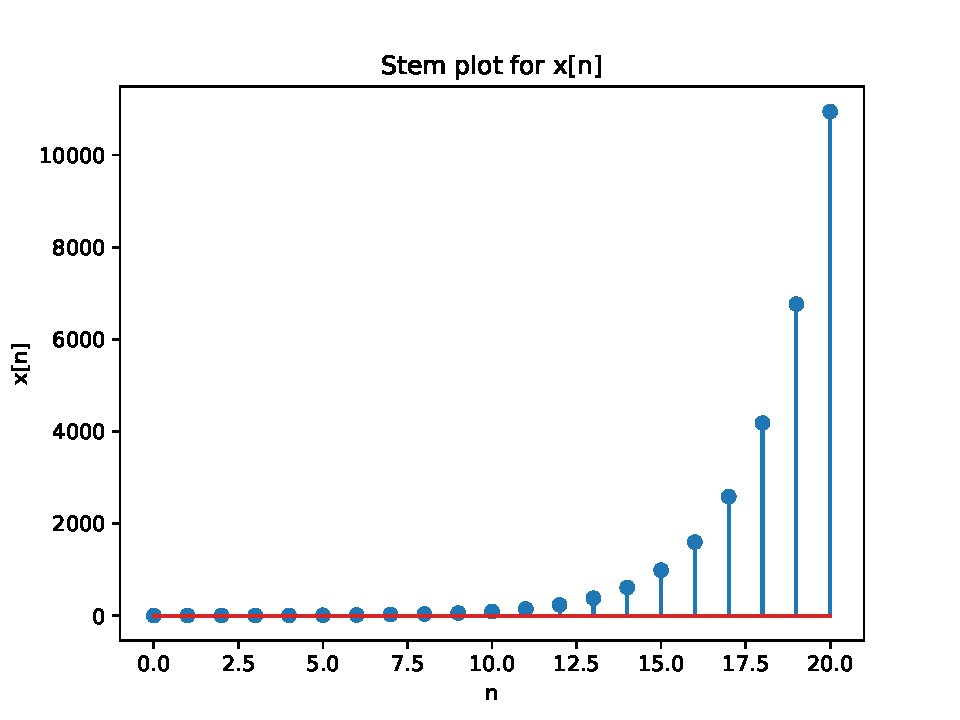
\includegraphics[width=0.45\textwidth]{./figs/2_2.pdf}
	\caption{Stem plot of $x[n]$}
	\label{fig:2_2}
\end{figure}
\item Find $X^{+}(z)$.\\
\solution
\begin{align}
\mathcal{Z}^+\sbrak{x(n + 2)} = \mathcal{Z}^+\sbrak{x(n + 1)} + \mathcal{Z}^+\sbrak{x(n)} 
\end{align}
\begin{align}
&z^2(X^+(z) - x(0)) - zx(1) = (z+1)(X^+(z)) - zx(0)
\end{align}

\begin{equation}
\brak{z^2 - z - 1}X^+(z) = z^2 \\
\end{equation}

\begin{flalign}
X^+(z) &= \frac{1}{1 - z^{-1} - z^{-2}} &&
% X^+(z) &= \frac{1}{\brak{1 - \alpha z^{-1}}\brak{1 - \beta z^{-1}}}
\label{eq:X-z}
\end{flalign}

\item Find $x(n)$.\\
\solution
Using one-sided Z-transform $X^+(z)$, we can find the signal $x(n)$ using inverse Z-transform 
\begin{align}
	X^+(z) &= \frac{1}{1 - z^{-1} - z^{-2}} \\
	X^+(z) &= \frac{1}{\brak{1 - \alpha z^{-1}}\brak{1 - \beta z^{-1}}} \\
	X^+(z) &= \cfrac{\brak{\frac{\alpha}{\alpha - \beta}}}{1 - \alpha z^{-1}} + \cfrac{\brak{\frac{- \beta}{\alpha - \beta}}}{1 - \beta z^{-1}} 
\end{align}

Applying inverse $Z$-transform and using 
\begin{equation}
a^n u(n) \stackrel{\mathcal{Z}}{\rightleftharpoons} \frac{1}{1 - \alpha z^{-1}}
\end{equation}

We have
\begin{align}
	x(n) &= \brak{\frac{\alpha}{\alpha - \beta}} {\alpha}^{n} u[n] - \brak{\frac{\beta}{\alpha - \beta}} {\beta}^{n} u[n] \\
	x(n) &= \brak{\cfrac{{\alpha}^{n+1} - {\beta}^{n+1}}{\alpha - \beta}} u[n]
	\label{eq:x_n}
\end{align}

\item Sketch 
\begin{align}
	y(n)	 = x\brak{n-1} + x\brak{n+1},  \quad n \ge 0
	\label{eq:10-orig-diff-rev}
\end{align}

\solution
Download the following python code for the stem plot of $y[n]$
\begin{lstlisting}
	wget 2_5.py
\end{lstlisting}
\begin{figure}[!ht]
	\centering
	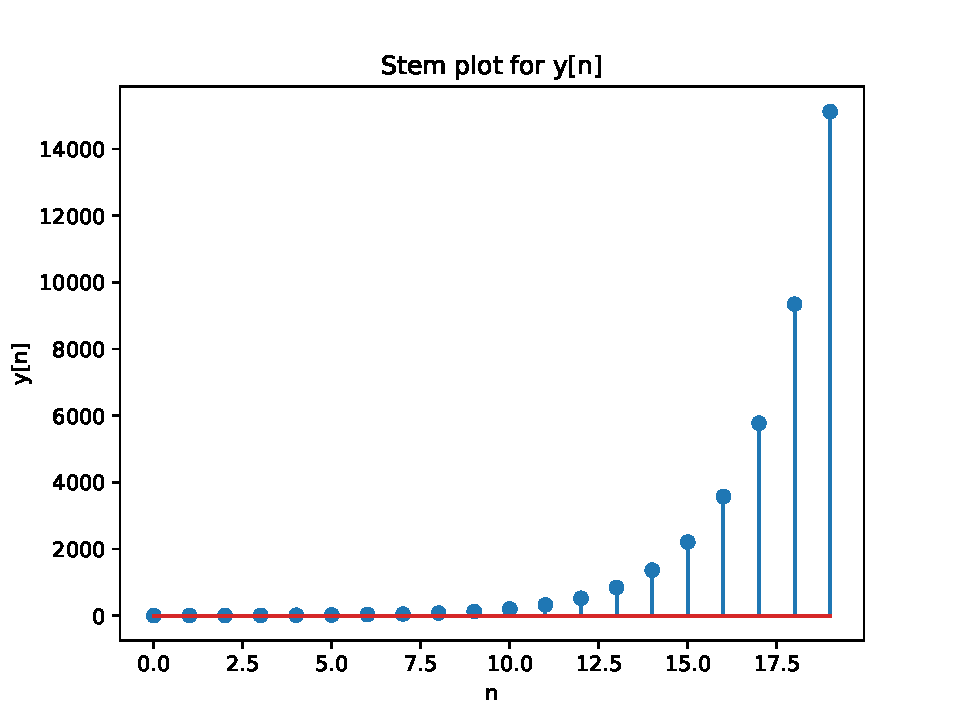
\includegraphics[width=0.45\textwidth]{./figs/2_5.pdf}
	\caption{Stem plot of $y[n]$}
	\label{fig:2_5}
\end{figure}

\item Find $Y^{+}(z)$.

\solution Taking the one-sided $Z$-transform on both sides of \eqref{eq:10-orig-diff-rev},
\begin{align}
&\mathcal{Z}^+\sbrak{y(n)} = \mathcal{Z}^+\sbrak{x(n + 1)} + \mathcal{Z}^+\sbrak{x(n - 1)} 
\end{align}

\hspace{3mm} Using $x(n) = 0\ \forall\ n < 0$ and the one-sided $Z$-transform, 

\begin{align}
Y^+(z) &= zX^+(z) - zx(0) + z^{-1}X^+(z) \\
&= \frac{z + z^{-1}}{1 - z^{-1} - z^{-2}} - z \\
&= \frac{1 + 2z^{-1}}{1 - z^{-1} - z^{-2}}
\label{eq:Y-z}
\end{align}

\item Find $y(n)$ \\
\solution
Factor the one-sided $Z$-transform as follows,
\begin{align}
	Y^+(z) &= \frac{1 + 2z^{-1}}{1 - z^{-1} - z^{-2}}\\
	&= \frac{1 + 2z^{-1}}{(1 - \alpha z^{-1})(1 - \beta z^{-1})}\\
	&= \frac{\brak{\frac{\alpha + 2}{\alpha - \beta}}}{1 - \alpha z^{-1}} - \frac{\brak{\frac{\beta + 2}{\alpha - \beta}}}{1 - \beta z^{-1}} \\
	&= \brak{\frac{1}{\alpha - \beta}} \brak{\frac{\alpha + 2}{1 - \alpha z^{-1}} - \frac{\beta + 2}{1 - \beta z^{-1}}} 
\end{align}
Applying inverse $Z$-transform, 
\begin{align}
	y(n) &= \frac{(\alpha + 2)({\alpha}^n u[n]) - (\beta + 2)({\beta}^n u[n])}{\alpha - \beta} \\
	&= \frac{{\alpha}^{n+1} - {\beta}^{n+1} + 2 \brak{\alpha^n - \beta^n}}{\alpha - \beta} \cdot u[n] \\
	&= \frac{{\alpha}^{n+1} - {\beta}^{n+1}}{\alpha - \beta} \cdot u[n] + \frac{2 \brak{\alpha^n - \beta^n}}{\alpha - \beta} \cdot u[n] \\
	&= x(n) + 2 x(n-1)\\
	&= (x(n) + x(n-1)) + x(n-1) 
\end{align}
The final expression for $y(n)$ is given by 
\begin{align}
	y(n) &= x(n+1) + x(n-1) \quad n > 0
	\label{eq:y_n}
\end{align}
\end{enumerate}

\section{Power of the Z transform}
\begin{enumerate}[label=\thesection.\arabic*,ref=\thesection.\theenumi]
\item Show that 
\begin{align}
	\sum_{k=1}^{n}a_k = 
	\sum_{k=0}^{n-1}x(k) = x(n)*u(n-1)
	\label{eq:an_xn_conv}
\end{align}

\solution
We observe the following relation from the expressions for $a[n]$ and $x[n]$

\begin{align}
	a[n]u[n] &= \brak{\frac{{\alpha}^n - {\beta}^n}{\alpha - \beta}}u[n]\\
	x(n) &= \brak{\frac{{\alpha}^{n+1} - {\beta}^{n+1}}{\alpha - \beta}}u[n]
\end{align}

So, $a[n+1] \cdot u[n] = x(n)$

\begin{flalign} 
	\sum_{k=1}^{n}a_k = \sum_{k=1}^{n}x(k - 1) 
\end{flalign}
Replacing $k$ with $k+1$ in the above expression 
\begin{flalign}
\sum_{k=1}^{n}a_k &= \sum_{k=0}^{n-1}x(k + 1 - 1) \\
\sum_{k=1}^{n}a_k &= \sum_{k=0}^{n-1}x(k) 
\end{flalign}

By the definition of convolution, 

\begin{align} 
	x(n) * u(n-1) &= \sum_{k=0}^{n-1}x(k)u(n-1-k) \\
	&= \sum_{k=0}^{n-1}x(k)u(n-k) 
\end{align}
\begin{align}
	u(n-k) > 0, \hspace{4mm}k = 0 \dots n-1
\end{align}
\begin{equation}
	x(n)*u(n-1) = \sum_{k=0}^{n-1}x(k)
\end{equation}

Hence, we have the final result
\begin{equation}
	\sum_{k=1}^{n}a_k = \sum_{k=0}^{n-1}x(n) = x(n)*u(n-1)
\end{equation}

\item Show that 

\begin{align}
a_{n+2}-1, \quad n \ge 1
\end{align}
can be expressed as 
\begin{align}
	\sbrak{x\brak{n+1}-1}u\brak{n}
\end{align}

\solution 

Using \eqref{eq:x_n}, we have
\begin{align} 
	x(n) = a(n+1) \quad n \ge 0
\end{align}
\begin{align}
    a_{n+2} - 1 = x(n + 1) - 1
\end{align}
and from the definition of $u[n]$,
\begin{align}
    a_{n+2} - 1 = \sbrak{x(n + 1) - 1} \times u[n]
\end{align}

\item Show that 
\begin{align}
	\sum_{k=1}^{\infty}\frac{a_k}{10^k}= 
	\frac{1}{10}\sum_{k=0}^{\infty}\frac{x\brak{k}}{10^k} =\frac{1}{10}X^{+}\brak{{10}}
\end{align}

\solution
Using \eqref{eq:x_n}, we have
\begin{align}
	x(n) = a(n+1) \quad n \ge 0
	\label{eq:xn_an}
\end{align}

\begin{align}
	\sum_{k=1}^{\infty}\frac{a_k}{10^k} &= \sum_{k=1}^{\infty}\frac{x(k-1)}{10^k} \\
	&= \sum_{k=0}^{\infty}\frac{x(k + 1 - 1)}{10^{k+1}} \\
	&= \frac{1}{10}\sum_{k=0}^{\infty}\frac{x(k)}{10^k} 
\end{align}
Using the definition of $X^{+}\brak{z}$, we have
\begin{align}
	\sum_{k=1}^{\infty}\frac{a_k}{10^k} &= \frac{1}{10}X^{+}\brak{{10}}
	\label{eq:ak_10}
\end{align}

\item Show that 
\begin{align}
	\alpha^n + \beta^n, \quad n \ge 1
\end{align}
can be expressed as 
\begin{align}
	w(n) =\brak{\alpha^{n+1} + \beta^{n+1}}u(n)
\end{align}
		and find $W(z)$.

\solution
\begin{align}
	{\alpha}^n + {\beta}^n \quad n \ge 1
\end{align}
Replace $n$ with $n+1$ in the above expression
\begin{align}
	{\alpha}^{n+1} + {\beta}^{n+1} \quad n \ge 0 \\
	\text{Also, } u[n] = 1 \quad n \ge 0 
\end{align}
So, the given expression can be written as
\begin{align}
	\brak{{\alpha}^{n+1} + {\beta}^{n+1}} \cdot u[n] 
\end{align}
\begin{align}
	W(z) &= \mathcal{Z}\brak{\brak{{\alpha}^{n+1} + {\beta}^{n+1}} \cdot u[n]} \\
	&= \mathcal{Z}\brak{{\alpha}^{n+1} \cdot u[n]} + \mathcal{Z}\brak{{\beta}^{n+1} \cdot u[n]} \\
	&= \frac{\alpha}{1 - \alpha z^{-1}} + \frac{\beta}{1 - \beta z^{-1}} \\
	&= \frac{\alpha + \beta - 2\alpha \beta z^{-1}}{1 - \alpha z^{-1} - \beta z^{-1} + \alpha \beta z^{-2}} 
\end{align}
Using $\alpha + \beta = 1$ and $\alpha \beta = -1$
\begin{align}
	W(z) = \frac{1 + 2z^{-1}}{1 - z^{-1} - z^{-2}}
\end{align}
\item Show that 
\begin{align}
	\sum_{k=1}^{\infty}\frac{b_k}{10^k} =
	\frac{1}{10}\sum_{k=0}^{\infty}\frac{y\brak{k}}{10^k} =\frac{1}{10}Y^{+}\brak{{10}}
\end{align}
\solution
\\Using \eqref{eq:y_n} and \eqref{eq:xn_an}, we have
\begin{align}
	y(n) &= x(n+1) + x(n-1) \\
	y(n) &= a(n+2) + a(n) \\
	y(n) &= b(n+1)
	\label{eq:yn_bn}
\end{align}
Now, using \eqref{eq:yn_bn}, we have
\begin{align}
	\sum_{k=1}^{\infty}\frac{b_k}{10^k} &= \sum_{k=1}^{\infty}\frac{y(k-1)}{10^k} \\
	&= \sum_{k=0}^{\infty}\frac{y(k + 1 - 1)}{10^{k+1}} \\
	&= \frac{1}{10}\sum_{k=0}^{\infty}\frac{y(k)}{10^k}
\end{align}
From the definition of one-sided $Z$-transform, we have
\begin{align}
	\frac{1}{10}\sum_{k=0}^{\infty}\frac{y(k)}{10^k} = \frac{1}{10}Y^{+}\brak{{10}}
	\label{eq:bk_10}
\end{align}
\item Solve the JEE 2019 problem. \\
\solution \\
\textbf{Option - (A) : True}
\begin{align}
	\sum_{k=1}^{n}a_k = a_{n+2}-1, \quad n \ge 1
\end{align}
\begin{align}
	&\mathcal{Z}(x(n)*u(n-1)) = \mathcal{Z}(x(n)) \cdot \mathcal{Z}(u(n-1)) \\
	&= X^+ (z) \cdot \frac{z^{-1}}{1-z^{-1}} \\
	&= \frac{z^{-1}}{(1 - z^{-1})(1 - z^{-1} - z^{-2})} \\
	&= z \brak{\frac{1}{1 - z^{-1} - z^{-2}} -\frac{1}{1 - z^{-1}}} \\
	&= z \sum_{n = 0}^{\infty} \brak{x(n) - 1} z^{-n} \\
	&= \sum_{n = 1}^{\infty} \brak{x(n) - 1} z^{1-n} \quad ,x(0) = 1 \\
	&= \sum_{n = 0}^{\infty} \brak{x(n+1) - 1} z^{-n} \\
	&= \mathcal{Z}(x(n+1) - 1)u(n) \\
	&\text{So, } (x(n)*u(n-1)) = (x(n+1) - 1) \quad n \geq 0
\end{align} 
From \eqref{eq:an_xn_conv}, we have 
\begin{align}
	\sum_{k=1}^{n}a_k &= x(n) * u(n-1) \\
	&= x(n+1) - 1 \\
	&= a_{n+2} - 1
\end{align}
\textbf{Option - (B) : True}
\begin{align}
	\sum_{n=1}^{\infty} \frac{a_n}{10^n} = \frac{10}{89}
\end{align}
From \eqref{eq:X-z} and \eqref{eq:ak_10}, we have
\begin{align}
	&\sum_{k=1}^{\infty}\frac{a_k}{10^k} = \frac{1}{10}X^{+}\brak{{10}} \\
	&X^+(10) = \frac{1}{1 - \frac{1}{10} - \frac{1}{100}} = \frac{100}{89} \\
	&\sum_{k=1}^{\infty}\frac{a_k}{10^k} = \frac{1}{10} \cdot \frac{100}{89} = \frac{10}{89}
\end{align}
\textbf{Option - (C) : False}
\begin{align}
	\sum_{n=1}^{\infty} \frac{b_n}{10^n} = \frac{10}{89}
\end{align}
From \eqref{eq:Y-z} and \eqref{eq:bk_10}, we have
\begin{align}
	&\sum_{k=1}^{\infty}\frac{b_k}{10^k} = \frac{1}{10}Y^{+}\brak{{10}} \\
	&Y^+(10) = \frac{1 + \frac{2}{10}}{1 - \frac{1}{10} - \frac{1}{100}} = \frac{120}{89} \\
	&\sum_{k=1}^{\infty}\frac{b_k}{10^k} = \frac{1}{10} \cdot \frac{120}{89} = \frac{12}{89}
\end{align}
\textbf{Option - (D) : True}
\begin{align}
	b_n = \alpha^n + \beta^n \quad n \geq 1
\end{align}
From definitions of $a_n$ and $b_n$, we have
\begin{align}
	b_n &= a_{n-1} + a_{n+1} \quad n \geq 2\\
	&= \frac{\alpha^{n-1} + \alpha^{n+1}}{\alpha - \beta} - \frac{\beta^{n-1} + \beta^{n+1}}{\alpha - \beta} \\
	&= \frac{\brak{\alpha^n + \beta^n}\brak{\alpha-\beta}}{\alpha - \beta} = \alpha^n + \beta^n 
\end{align}
Using $b_1 = 1 \text{ and } \alpha + \beta = 1$ \\
So, 
\begin{align}
b_n = \alpha^n + \beta^n \quad n \geq 1
\end{align}
\end{enumerate}
\end{document}
